\documentclass{turabian-thesis}

\usepackage{graphicx}
\usepackage{subcaption}
\usepackage{pslatex}
\usepackage{amsthm}
\usepackage{amsmath}
\usepackage{amssymb}
\usepackage{mathtools}
\usepackage{bm}
\usepackage{paralist}
\usepackage[utf8]{inputenc}
\usepackage{multicol} 
\usepackage[hidelinks]{hyperref}
\usepackage{nameref}
\usepackage{setspace}
\usepackage{listings}

\usepackage[toc,page]{appendix}


\DeclareUnicodeCharacter{2215}{\textminus}
\usepackage{algorithm}
\usepackage{algpseudocode}
\algdef{SE}[DOWHILE]{Do}{DoWhile}{\algorithmicdo}[1]{\algorithmicwhile\ #1}%

\newtheorem{theorem}{Theorem}
\newtheorem{lemma}{Lemma}
\newtheorem{corollary}{Corollary}
\newtheorem{claim}{Claim}
\newtheorem{definition}{Definition}
\newtheorem{problem}{Problem}

\newcounter{case}[section]
\newenvironment{case}[1][]{\refstepcounter{case}\par\medskip
   \textbf{Case~\thecase. #1} \rmfamily}{\medskip}
   
\newcounter{subcase}[case]
\newenvironment{subcase}[1][]{\refstepcounter{subcase}\par\medskip
   \textbf{Case~\thecase.\thesubcase. #1} \rmfamily}{\medskip}

\begin{document}

\frontmatter
\thispagestyle{empty}

\begin{center}
   
   \textbf{Hybrid Model for Interpretable Time Series Analysis}
   
   \vspace*{\baselineskip} 
      
   A THESIS \\
   Presented to the Department of Computer Science and Computer Engineering \\
   California State University, Long Beach
   
   \vspace*{\baselineskip} 

   In Partial Fulfillment \\
   of the Requirements for the Degree \\
   Master of Science in Computer Science \\
   Option in Computer Science
   
   \vspace*{\baselineskip} 

   Committee Members: \\
   Ju Cheol Moon, Ph.D \\
   Roman Tankelevich, Ph.D \\
   Seok-Chul Kwon, Ph.D

   \vspace*{\baselineskip} 

   College Designee: \\
   Hamid Rahai, Ph.D.
   
   \vspace*{\baselineskip} 

   By Ruben Rosales \\
   May 2020
\end{center}

\pagebreak

\chapter*{Abstract}

% In this thesis, we study interpretable machine learning as applied to complex-valued time series data. Scientists have studied the use of several machine learning methods such as Convolutional Neural Networks, Recurrent Neural Networks, and Support Vector Machines for time series classification. These methods, however, fall short of allowing users to visualize patterns within their dataset.

% To address this issue, we propose an interpretable hybrid model that can be extended to any time series dataset. Our architecture is composed of two models, an ensemble method of classifiers that functions as a black-box model, and a white-box model that encodes time series as an image, attempts to classify them through a CNN, and outputs all images correctly classified in both black-box and white-box models.

In this thesis, we study interpretable machine learning as applied to complex-valued time-series data. Scientists have studied the use of several machine learning methods such as Convolutional Neural Networks, Recurrent Neural Networks, and Support Vector Machines for time series classification. These methods, however, fall short of allowing users to visualize patterns within their dataset.

To address this issue, we propose an interpretable hybrid model that can be extended to any time series dataset. In the majority of existing work in the field of interpretability, black-box models tend to outperform white-box models consistently. However, instead of relying purely on one method, we propose a collaboration between the two. This allows for the performance of a black-box model while providing a more precise visualization of our dataset.

To accomplish this, we created a framework composed of two models, an ensemble method of classifiers that functions as a black-box model, and a white-box model that encodes time series as images. The white-box model attempts to classify them through a neural network and outputs all images correctly classified in both black-box and white-box models.

\addcontentsline{toc}{chapter}{Abstract}
\chapter{Acknowledgments}

I want to thank Dr. Moon for his guidance and for allowing me to work on a project this extensive. I would also like to thank my friends and family for their continuous support throughout this thesis.

\tableofcontents
\listofillustrations

\mainmatter
\chapter{Introduction}
\label{chap:introduction}

As time-series datasets become ever more popular, the need for deep learning models becomes that much greater. In our black-box model, we analyze deep learning models such as Convolutional Neural Networks, which have become increasingly popular and widely used in the last decade  \cite{cui_multi-scale_2016}. However, their complex nature results in a lack of understanding of its inner workings \cite{wang_hybrid_2019}.
As the use and complexity of black-box models rises, so too does the need for an interpretable accessory. For this reason, we propose a hybrid model consisting of a black-box for classification and an interpretable white-box which highlights characteristics of a time series for users to understand.

The goal of our work is not to find an alternative to black-box models, but to provide a way for users to have an understanding of what features are prevalent in their dataset.

\begin{figure}[h!]
   \begin{center}
      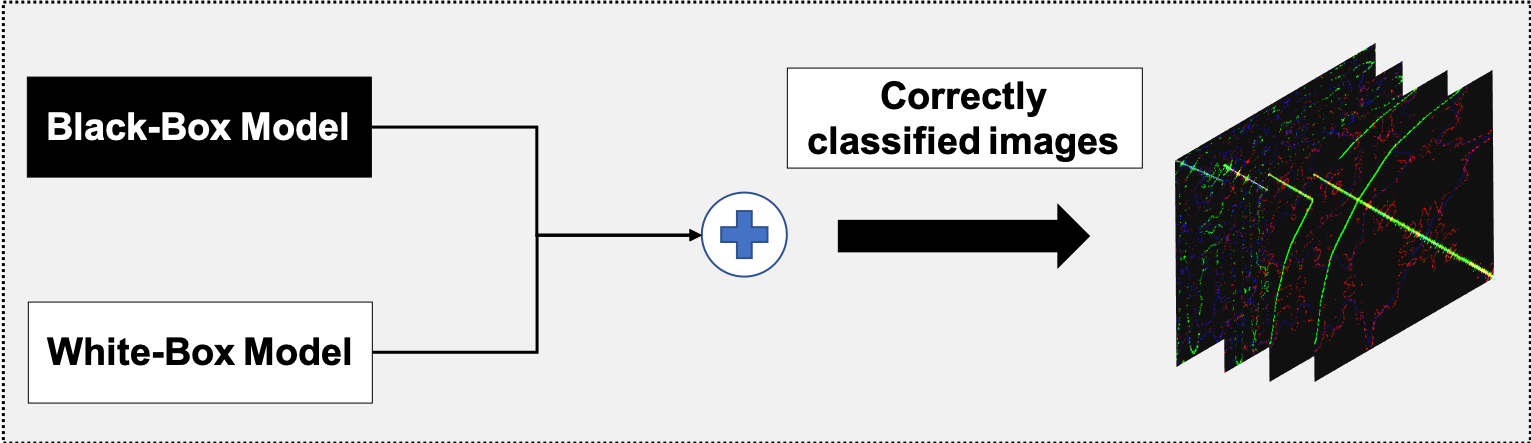
\includegraphics[scale=0.5]{../media/overview_model.png}
   \end{center}
   \caption{Overview of our proposed hybrid model.}
   \label{fig:overview_model}
\end{figure}

% \section{The need for interpretable models in management problems}
% The growth of mobile devices and demand for wireless data has created a need for igh quality spectrum sensing and adaptation to improve spectral allocation and interference mitigation is an important route by which we may achieve this.  however have been constrained to relatively specialized solutions which lack the generality needed to deal with a complex and growing number emitter types, interference types and propagation environments.
% This is a significant challenge in the community as expert systems designed to perform well on specialized tasks often lack flexibility and can be expensive and tedious to develop analytically.

\section{Contributions}
We focus on creating deep learning architectures to classify our datasets as well as extending existing work to create our white-box model. Our final results show how robust our black-box model is with its competitive accuracy. Additionally, we show the effectiveness of our white-box model in understanding the features of a dataset not normally exposed through a black-box model.


\chapter{Data}

We analyzed our model on three radio signal datasets, which we will refer to as dataset A, B, and C throughout this thesis. These datasets were generated through Spatial Modulation which is a transmission technique that uses multiple antennae which maps a block of information bits to two units, a symbol chosen from a constellation diagram, and a unique transmit antenna number that is chosen from a set of transmit antennae \cite{mesleh_spatial_2008}. The method in which transmit antennae send and receive radio waves can be described through polarization. Two popular basis polarizations are horizontal linear, H, and vertical linear, V \cite{oshea_convolutional_2016}. Our datasets contain data horizontally transmitted and vertically received (HV), as well as data vertically transmitted and vertically received (VV).

\begin{figure}[h!]
   \begin{center}
      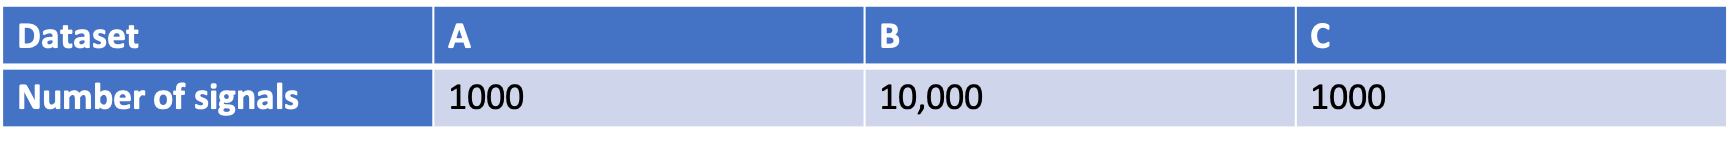
\includegraphics[scale=0.5]{../media/dataset_info.png}
   \end{center}
   \caption{Size of each dataset.}
   \label{fig:dataset_info}
\end{figure}

The two properties, HV and VV, are given to us in a raw and discrete format. Both properties consist of time and amplitude values but vary in length and in how they are processed. The raw signal consists of over 31,000 data points with the exact time it was received. The size of the discrete data can vary from 22 to 44 data points and is a processed representation of the raw signal that has equally spaced values. In this thesis, we focus on discrete data given that it is closer to datasets in real-world situations.

\section{Dataset Classes}

Dataset A and C were generated through similar methods and can be visually seen in Figure \ref{fig:dataset_ac}. There are three base stations, in which each base station corresponds to a class, sending information to a single receiver antenna.


\begin{figure}[h!]
   \begin{center}
      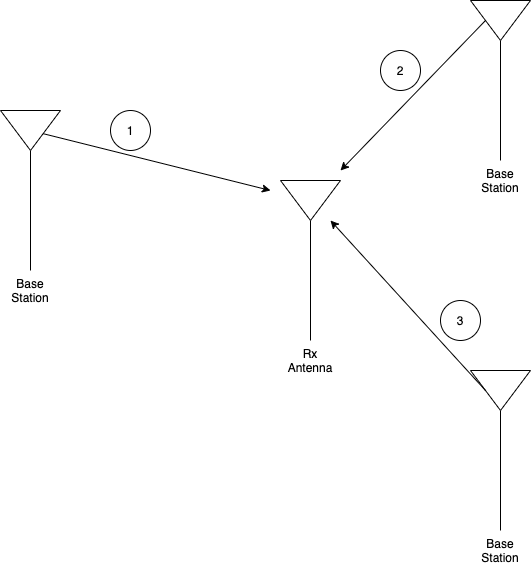
\includegraphics[scale=0.4]{../media/dataset_ac.png}
   \end{center}
   \caption{Class representation of how dataset A and C.}
   \label{fig:dataset_ac}
\end{figure}

Dataset B differs from dataset A and C in how it transmits data. In \ref{fig:dataset_b}, we can see that there are three different antennas at the same station sending information to a single receiver station. The problem of classification becomes more challenging because they are very close together.

\begin{figure}[h!]
   \begin{center}
      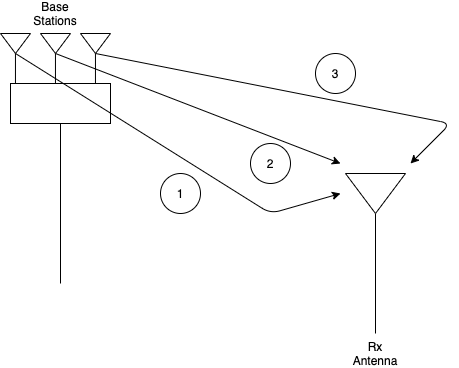
\includegraphics[scale=0.5]{../media/dataset_b.png}
   \end{center}
   \caption{Class representation of how dataset B.}
   \label{fig:dataset_b}
\end{figure}


% [ What is raw signal and discrete, compare them, ]
% [explain hv, vv]

\chapter{Related Work}
\label{chap:relatedwork}

The study of interpretable hybrid models has been worked on extensively in the past few years as deep learning has become increasingly popular. Scientists take different approaches as to what makes a hybrid model interpretable and apply it to different domains, such as computer vision or time series. For example, in \cite{wang_multilevel_2018}, they focus on creating a black-box model for the classification of time-series that outperforms similar architectures. However, their white-box model focuses on analyzing the importance of their model's layers. This helps users identify the importance of wavelet decomposition but not necessarily understand their dataset. 

Additionally, other work we found tends to focus on non-time-series data or creating a general framework defining the trade-off between interpretability and black-box methods. For instance, \cite{wang_hybrid_2019} defines a set of rules to achieve a high level of classification with interpretability but does not give any competitive methods to achieve this. 

In order to fill the gap for a high performing interpretable model for time-series classification, we propose our hybrid model, which focuses on extensibility and robustness. We achieve this through a combination of deep learning models for classification as well as a unique white-box method to explaining features within classes of a given dataset.


\chapter{Preprocessing}
\label{chap:preprocessing}

The radio signal data is presented in a complex-valued format that is unusable in a typical neural network, so in an attempt to make our model robust and reduce any complexity, we focused on using real values as features.

We tried numerous methods to extract real-valued features, including Fourier Transform, Short-Time Fourier Transform, a custom sliding window method, and polar coordinates taken directly from the signal's amplitude/phase value. Before applying any of these methods, we normalized all data using L2 normalization.

% \section{What is it?}
% [what is feature extraction]

% % maybe?
% % Data pre-processing is concerned with the analysis and manipulation of the collected spectrum data to arrive at potentially good wireless data representations. The raw samples organized into data vectors rk in the previous block are pipelined as input for signal processing (SP) tools that analyze, process and transform the data to arrive at simple data representations such as frequency,
% % amplitude, phase and spectrum, or more complex features
% % xk such as e.g. cyclostationary features. In addition, feature
% % learning such as deep learning may be utilized to automatically
% % extract more low-level and high-level features. In many ML
% % applications the choice of features is just as important, if not
% % more important than the choice of the ML algorithm.


\section{Transformations}


\subsection{Fourier Transform}
% [Recall we can write a complex number in terms of its magnitude and phase
% (i.e., its polar representation). ]

% Transformation 1 : STFT/ FT
% [what is it]

% [fft formula]
The Fourier Transform (FT) is a mathematical tool that decomposes any function into a sum of sinusoidal basis functions. Each basis function is a complex value of a frequency, allowing us to view our data in the frequency domain as opposed to the amplitude domain.

One of the shortcomings of the FT is rooted in the Heisenberg Uncertainty Principle (HUP) \cite{hill_uncertainty_nodate}.  The HUP states that the position and velocity of an object cannot be simultaneously measured, which can be applied to the time-frequency information of a signal. This means we cannot know which spectral components exist at any given time. The closest we can get is sampling at different ranges of time and finding a range of frequencies within that time frame. This method is described as the Short-Time Fourier Transform.


% The Fourier Transform is a magical mathematical tool. The Fourier Transform decomposes any function into a sum of sinusoidal basis functions. Each of these basis functions is a complex exponential of a different frequency. The Fourier Transform, therefore gives us a unique way of viewing any function - as the sum of simple sinusoids.

% The Fourier Series showed us how to rewrite any periodic function into a sum of sinusoids. The Fourier Transform is the extension of this idea to non-periodic functions.

% While the Fourier Transform is a beautiful mathematical tool, its widespread popularity is due to its practical application in virtually every field of science and engineering. It's hard to understand why the Fourier Transform is so important. But I can assure you it enables the solution to difficult problems be made simpler (and also makes previously unsolved problems solvable). In addition, the Fourier Transform gives us a new method of viewing the world, which is fantastic for giving a more intuitive feel for our universe.


\subsection{Short-Time Fourier Transform}
% [stft]
The Short-Time Fourier transform (STFT) is a Fourier related transform used to determine the sinusoidal frequency and phase content of local sections of a signal as it changes over time \cite{hill_uncertainty_nodate}.
Computing STFT requires the signal to be divided into segments of equal length and then have the FT applied to that segment \cite{allen_unified_1977}. This allows us to view the Fourier spectrum at a more granular level, which could potentially reveal different patterns amongst signals of different classes.


One of the issues with this method is that we can create very narrow window sizes, giving us a better understanding of the data with respect to time but losing an understanding of the frequency domain as a whole. Additionally, selecting an appropriate window size for segmenting the signal can be an arduous task that would require fine-tuning as well as increasing the dimensionality of a dataset.


\begin{figure}[h]
   \begin{center}
      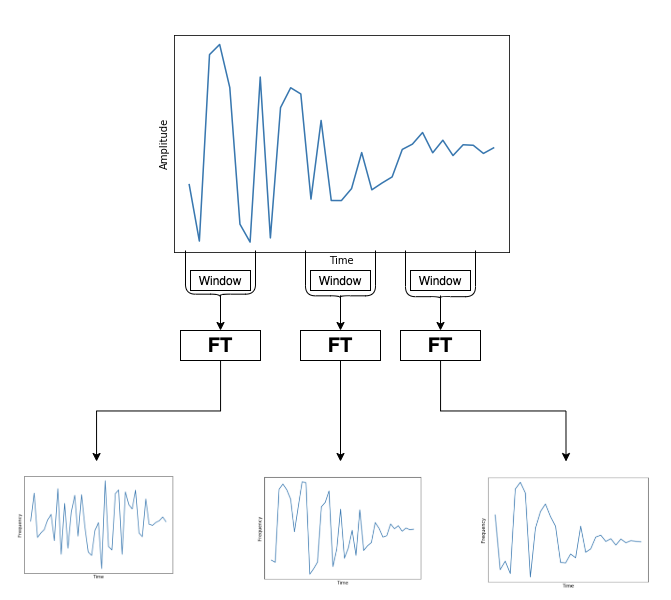
\includegraphics[scale=0.6]{../media/stft.png}
   \end{center}
   \caption{Example of Short-Time Fourier Transform.}
   \label{fig:stft_example}
\end{figure}

% The problem with STFT is the fact whose roots go back to what is known as the Heisenberg
% Uncertainty Principle. This principle originally applied to the momentum and location of
% moving particles, can be applied to time-frequency information of a signal. Simply, this principle
% states that one cannot know the exact time-frequency representation of a signal, i.e., one cannot
% know what spectral components exist at what instances of times. What one can know are the
% time intervals in which certain bands of frequencies exist, which is a resolution problem.
% The problem with the STFT has something to do with the width of the window function that is
% used. To be technically correct, this width of the window function is known as the support of
% the window. If the window function is narrow, then it is known as compactly supported. This
% terminology is more often used in the wavelet world, as we will see later.

% The problem is that when you are studying a real signal it would be useful to know what the ‘instantaneous frequency’ of the signal is. The instantaneous frequency is the exact frequency of a signal at an exact moment in time. For instance if I was listening to a music track I would like to be able to say ‘at 1 min 59.0423 seconds into the music track the so,und is 1563.2 Hz’. Unfortunately the Fourier Transform cannot do this because there exists a minimum amount of uncertainty between the frequency and time domains, like Heisenberg has a minimum amount of uncertainty between the speed and position of a particle (the area of the box). You can know the moment in time you want to find the frequency for (like the blue box), but because there is a minimum uncertainty, the box of has to stretch out across frequency, meaning that you are unsure of the frequency at that moment in time.

% The best you can do with a Fourier Transform is to sample a range of time (for instance, the time signal between 1 min 58 sec and 1 min 59 sec in a song) and find a range of frequencies that were played over that amount of time, as represented by the black box. An example of this can be seen by looking at the third picture in the post again. There is a signal over a range of time (e.g. someone saying ‘hello’) and the frequency graph is the range of frequencies recorded over that time.



% [purpose and motivation? Behind making it ang/abs]

% [definition plus method]



\subsection{Sliding Window Method}

Similar to STFT, we segment our signal into N windows of equal length and perform FT on every segmentation. However, instead of keeping the output from FT, we only keep the mean value of each segmentation. This performed as well as STFT and gave us the advantage of reducing the dimensionality of our dataset. 

\subsection{Polar Coordinates}

% Transformation 2: Amplitude / Phase
The representation of a complex number as a sum of a real and imaginary number, z = x + iy, is called its Cartesian representation. For every cartesian point, we calculate its radius and angular distance as real values and use those as features. This method outperformed the previous three methods but limited our feature size, which made it difficult to get consistent accuracy across all three of our datasets.

\subsection{Wavelets}

Wavelet transforms are similar to the FT in that they deconstruct a signal using representations of other signals \cite{misiti_wavelets_2013}. The key difference is that wavelet signals are finite in time and frequency as opposed to sine and cosine signals, which can carry on indefinitely \cite{strang_wavelets_1996}. This allows us to extract information from a signal with respect to time and location.


\begin{figure}[h!]
   \begin{center}
      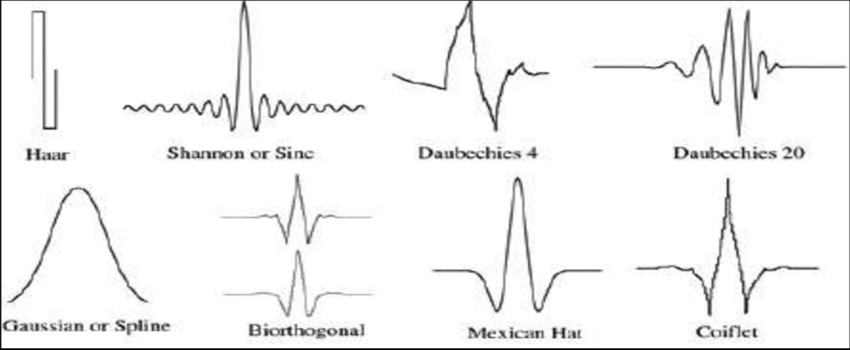
\includegraphics[scale=0.4]{../media/wavelet_families.png}
   \end{center}
   \caption{Example of different types of wavelets \cite{lopez_development_2017}.}
   \label{fig:reinforcementAgent}
\end{figure}


A signal is analyzed using different versions of dilated and translated basis functions called the mother wavelet  \cite{strang_wavelets_1996}. There are two types of wavelet transformations, discrete and continuous \cite{imani_curve_2016}. In this thesis, we focus on discrete wavelet transformations, which use a discrete set of wavelet scales and translations to decompose the signal into a mutually orthogonal set of wavelets. 

We take advantage of wavelets by applying discrete wavelet transforms as a filter-bank, meaning they are composed of cascading high-pass and low-pass filters. This allows us to split a signal into several frequency sub-bands  \cite{strang_wavelets_1996}. We focus on wavelet decomposition as our feature extractor because it outperformed all other methods in terms of accuracy and training time.

% Transformation 3: Wavelets

% Wavelets are similar to the FT in which they deconstruct a signal using representations of other signals. The key difference is wavelet signals are finite in time and frequency as opposed to sin and cos signals which can carry on forever. Simply, this allows us to extract information from a signal which respect to time and location.

% The use of wavelets is called the wavelet transform which is a technique in which a signal is analyzed using different versions of a dilated and translated basis functionss called the mother wavelet. There are two types of wavelet transformations, discrete and continous. In this thesis we focus on discrete.

% DWT uses a discrete set of wavelet scales and translations which decompose the signal into mutually orthogional set of wavelets.

% One advantage of wavelets is they have varying window sizes so they can be wide for slow frequencies and narrow for faster ones this is handled by the property called scale [add figure].

% wavelets 


% Some properties of wavelets are orthogonality, zero mean, and are efficient at representing localized data and functions.



% Db4 wavelet http://wavelets.pybytes.com/wavelet/db4/

% Model 1:
% Model 2: 
% Model 3: 



% In the preprocessing stage we tried numerous combinations of features but found the best performing features to come from wavelet decomposition.




% Wavelets

% We take advantage of wavelets by applying discrete wavelet transforms as a filter-bank which means it’s composed of cascading high-pass and low-pass filters. This gives us the advantage of splitting a signal into several frequency sub-bands. Wavelet decompositions give us the advantage of gaining features that take into account frequency and time domains. 

% [explain why they performed better]


% [alternatives]


\section{Data Shape}
% [Shape of data comparison]

A neural network requires all data to be the same shape. However, because we downsample in wavelet decomposition, our data size is halved, making it impossible to place all levels of decomposition into the same dataset. In order to circumvent this, we tested two different methods: resampling the data and treating each level of decomposition as a unique dataset.


\subsection{Resampling}

We use spline interpolation to resize each level of decomposition into a single array because it allows to retain properties of our original data even in a higher dimension \cite{gregory_shape_1985}. We tested different sizes of interpolation from N to N/3, where N is the size of the largest discrete signal size, and found no reduction in performance.
 
\subsection{Each Level of Decomposition as a Dataset}
Figure \ref{fig:multimodal_overview} depicts our model in which each level of decomposition is a unique dataset. This method and the resampling method both achieved similar results, so we chose to move forward with this method.



\begin{figure}[h!]
   \begin{center}
      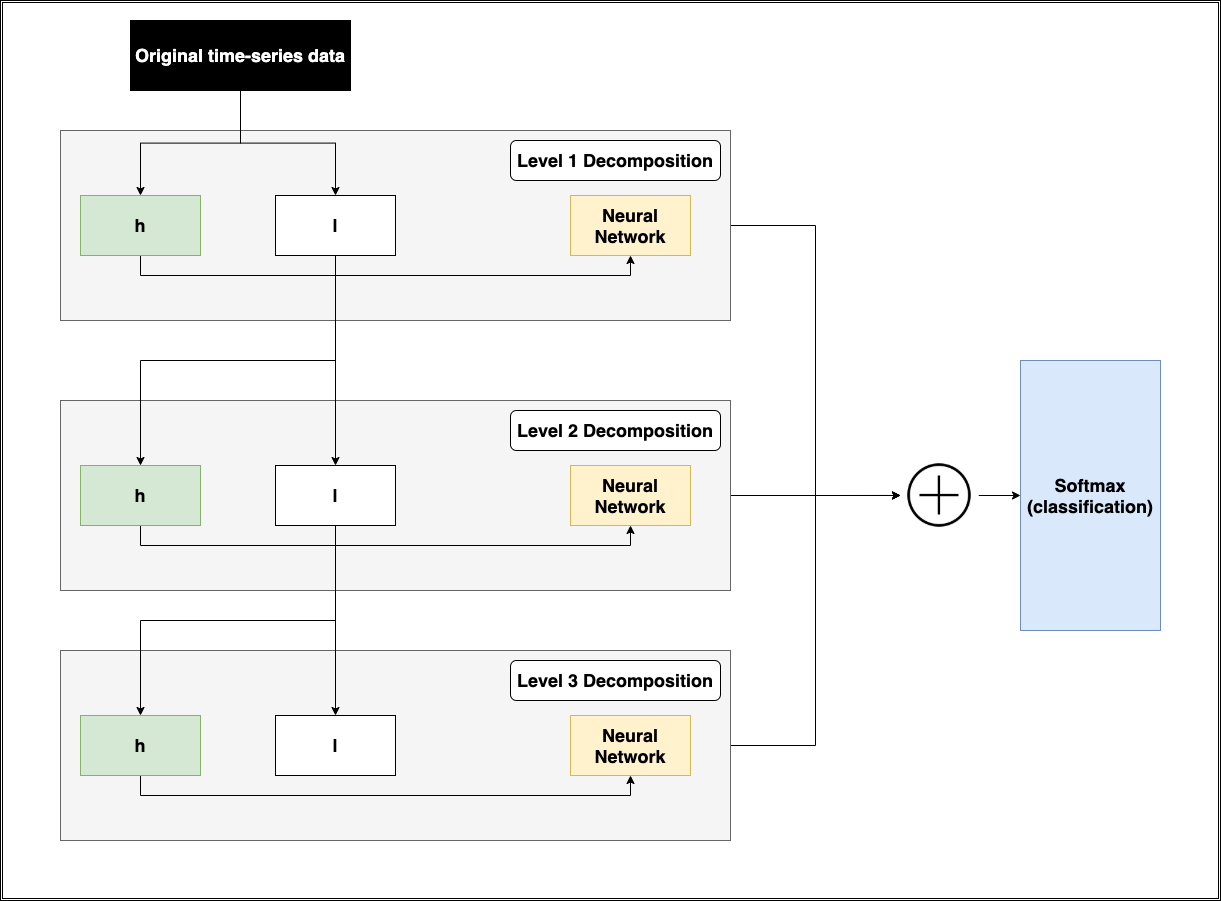
\includegraphics[scale=0.35]{../media/wavelet_decomp.png}
   \end{center}
   \caption{Example of a wavelet decomposition network.}
   \label{fig:wavelet_decomp}
\end{figure}


\chapter{Models}
\label{chap:models}

% [introduce models definitions]
% [EXPLAIN LOSS AND HOW ACCURACY IS MEASURED]


\section{Definition}
Machine learning algorithms can be seen as learning a target function (f) that maps input data (X) to an output (Y). There are several techniques to make this work, but we focus on nonparametric algorithms, namely Convolutional Neural Networks (CNN) and Long Short-Term Memory networks (LSTM). Nonparametric algorithms attempt to make minimal assumptions about the form of the function to learn any form from data provided to it. An example would be a neural network as it has no prior knowledge of what it is classifying and attempts to generalize any new data points.

\subsection{CNN}
% [cnn]

A Convolutional Neural Network is a type of deep neural network that can be applied to different domains such as computer vision or time series analysis. As seen in Figure X, it consists of an input and output layer as well as several hidden layers. A convolution is an operation between a vector of weights w against an input x \cite{yamashita_convolutional_2018}. It consists of taking the dot product between m and x in steps of a filter size defined by n.

Convolutional Neural Networks perform feature learning via non-linear transformations implemented as a series of layers \cite{aqib_smarter_2019}. The input data is a multidimensional array, called a tensor. The tensor is passed through an input layer, followed by a series of hidden layers to extract features, and an output layer, which in the case of classification, gives a probability for each class. 

% create your own design
\begin{figure}[h!]
   \begin{center}
      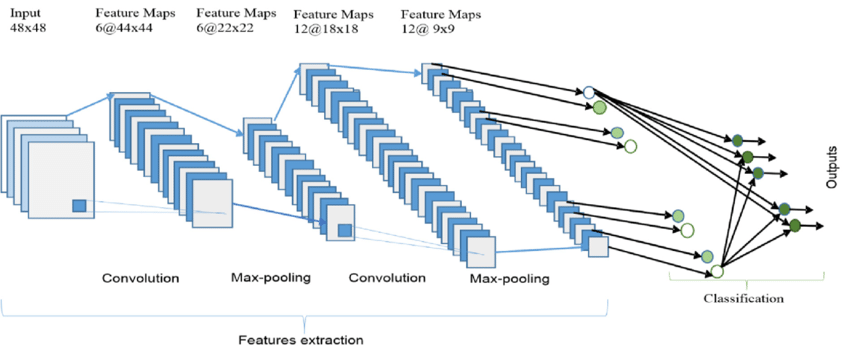
\includegraphics[scale=0.5]{../media/cnn_example.png}
   \end{center}
   \caption{Example of a Convolutional Neural Network \cite{alom_state---art_2019}.}
   \label{fig:cnn_example}
\end{figure}

Hidden layers are crucial to neural networks because they help in determining which data representations are useful for explaining the relationships in the given data. Each layer consists of several kernels,  which are feature detectors that convolve over the input data and output a transformed version of it. 



\subsection{LSTM}

% [lstm]
Long short-term memory (LSTM) is an artificial recurrent neural network (RNN) architecture used in the field of deep learning. Unlike standard feedforward neural networks, LSTM has feedback connections, processing not only single data points but also entire sequences of data. 

A standard LSTM unit is composed of a cell, an input gate, an output gate, and a forget gate. The cell remembers values over arbitrary time intervals, and the three gates regulate the flow of information into and out of the cell \cite{donahue_long-term_2016}.

LSTM networks are well-suited to classifying, processing, and making predictions based on time series data since there can be lags of unknown duration between significant events in a time series. LSTMs are developed to deal with the vanishing gradient problems that can are encountered when training traditional RNNs \cite{donahue_long-term_2016}. 

\begin{figure}[h!]
   \begin{center}
      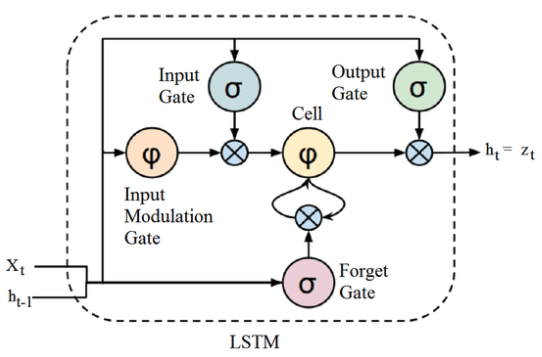
\includegraphics[scale=0.5]{../media/lstm_highlight.png}
   \end{center}
   \caption{Example of a LSTM unit \cite{donahue_long-term_2016}.}
   \label{fig:reinforcementAgent}
\end{figure}

\subsection{Multimodal Deep Learning}

% [multimodal]
Due to the superior performance and computationally tractable representation capability in multiple domains such as visual, audio, and text, deep neural networks have gained tremendous popularity in multimodal learning tasks \cite{kim_multimodal_2018}. Typically, domain-specific neural networks are used on different modalities to generate their representations, and the individual representations are merged or aggregated \cite{liu_learn_2018}. Finally, the prediction is made on top of aggregated representation, usually with another neural network to capture the interactions between models and learn complex function mapping between input and output.

% [explain architectures]

\section{Architectures Used}

\subsection{CNN}

Our CNN architecture consists of 3 convolutional layers each followed by a batch normalization and dropout layer then finally connected to a dense layer (Figure \ref{fig:cnn_model}). We attempted to make it deeper but found inconsistent performance across all of our datasets.
% [add figure]

\begin{figure}[h!]
   \begin{center}
      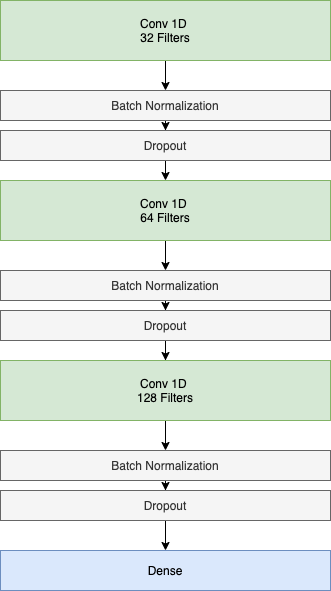
\includegraphics[scale=0.6]{../media/cnn_model.png}
   \end{center}
   \caption{CNN architecture used in our black-box model.}  
    \label{fig:cnn_model}
\end{figure}

\subsection{LSTM}
We wanted to keep our LSTM network as small as possible for simplicity, so we went with two LSTM layers of 128 hidden states and a dropout rate of 0.4  followed by a dense layer of 128 connections. We attempted different state sizes but found 128 to be the smallest number of units with the highest and most consistent rate of accuracy.

% [add figure]
\begin{figure}[h!]
   \begin{center}
      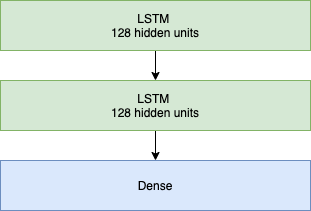
\includegraphics[scale=0.6]{../media/lstm_model.png}
   \end{center}
   \caption{LSTM architecture used in our black-box model.}
   \label{fig:lstm_model}
\end{figure}


\subsection{Final Model}

We propose a multimodal learning architecture for time series classification, which is illustrated in Figure \ref{fig:multimodal_overview}. The multimodal architecture allows our data to vary in size, and given that all three levels of decomposition have varying lengths due to downsampling, we propose that each model learn the representation of each distinct feature. For this model, we propose two architectures: a 1D CNN and an LSTM. We employ two CNN’s and one LSTM, with each concatenated following their respective dense layer, after which classification is performed via a softmax layer. 
% [add figure]

\begin{figure}[h!]
   \begin{center}
      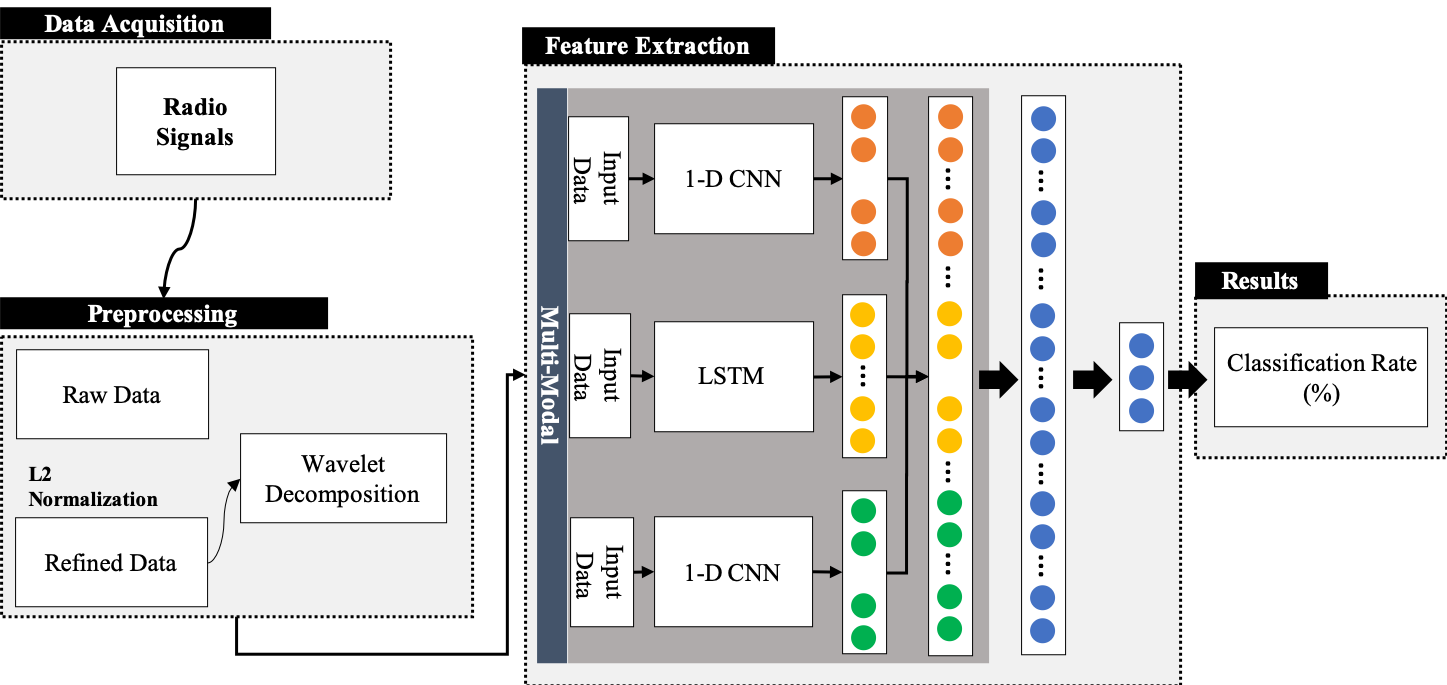
\includegraphics[scale=0.65]{../media/multimodal_overview.png}
   \end{center}
   \caption{Overview of our black-box model.}
   \label{fig:multimodal_overview}
\end{figure}


% \section{mtf}

% We approach our MTF is slightly different than  because instead of performing it over all samples in the dataset we perform it for every signal. 

% The three attributes we use are values are the absolute value of HV SBR, the absolute value of VV SBR, and a mathematical combination of the two (Figure X).

% [add figure]

 
\chapter{Markov Transition Fields}
\label{chap:mtf}

% We propose a framework similar to [] for encoding dynamical transition statistics,
% but we continue their work by considering ith order Markov transition probabilities.
% Given a time series X, we decompose its magnitude axis into two separate
% properties by representing it as a polar coordinate, Xangular and Xradial. We then
% identify the Q quantile bins for both properties and the temporal values Xtime
% and assign each x in Xangular, Xradial, Xtime to its corresponding bin qj (j in
% [1, Q]). Thus we construct three QxQ adjacency transition matrices, Wangular,
% Wradial, Wtime, by counting transitions among quantile bins in the manner of a
% ith order Markov chain along the time axis.

% W does not take into account the temporal axis so to prevent any information
% loss we construct a Markov Transition Field (MTF) for each W. The MTF
% denotes the probability of transitioning from qi to qj for each x in X. This,
% in turn, allows us to consider the transition probability on the magnitude and
% temporal axis.

% As described in [] the MTF encodes the multi-span transition probabilities
% of the time series, but given that we have three different M’s we modify their
% approach and consider each M to be a separate color channel of RGB where
% Mangular is red, Mtime is blue, Mradial is green. 

% \section{Markov Transition Field}
\section{Method}

We propose a framework similar to \cite{wang_encoding_nodate}  for encoding dynamical transition statistics, but we continue their work by adding i\textsuperscript{th} order Markov transition probabilities.

Given a time series X, we decompose its magnitude axis into three separate properties, P\textsubscript{1},  P\textsubscript{2},  P\textsubscript{3}. We then identify the Q quantile bins for each property  and assign each $x \in P\textsubscript{1},  P\textsubscript{2},  P\textsubscript{3}$ to its corresponding bin q\textsubscript{j} (j in [1, Q]). Thus, we construct three QxQ adjacency transition matrices, W\textsubscript{1}, W\textsubscript{2}, W\textsubscript{3}, by counting transitions among quantile bins in the manner of an i\textsuperscript{th} order Markov chain along the time axis.

\begin{figure}[h!]
   \begin{center}
      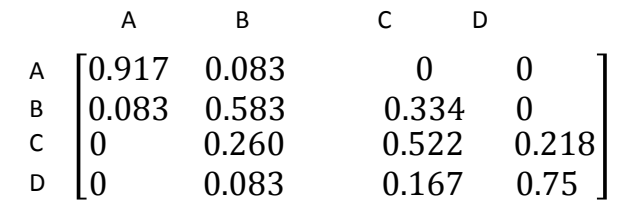
\includegraphics[scale=0.6]{../media/mtf_q.png}
   \end{center}
   \caption{Example of QxQ quantile bin matrix used to calculate MTF \cite{wang_encoding_nodate}.}
   \label{fig:mtf_q}
\end{figure}
 

%summation %. This effectively removes any sensitivity to the X’s distribution and temporal dependency to each time step t i. To account for any information loss after removing the temporal dependency, we follow the same approach as \cite{wang} and construct a Markov Transition Field for each property like so: %some figure%

W does not take into account the temporal axis, so to prevent any information loss, we construct a Markov Transition Field, M, for each W. The MTF denotes the probability of transitioning from q\textsubscript{i} to q\textsubscript{j} for each $x \in P$. This, in turn, allows us to consider the transition probability on the magnitude and temporal axis.

\begin{figure}[h!]
  \centering
  M =
  \[\begin{bmatrix}

  \text{W\textsubscript{ij}} | \text{$x\textsubscript{1} \in q\textsubscript{i}$, $x_{1} \in q\textsubscript{j}$}
  & \dots &
  
  \text{W\textsubscript{ij}}  |  \text{$x_{1} \in q\textsubscript{i}$, $x_{n} \in q\textsubscript{j}$} 
  
  \\
  
  \vdots &  \ddots & \\
  
  \text{W\textsubscript{ij}} | \text{$x_{n} \in q\textsubscript{i}$, $x_{1} \in q\textsubscript{j}$}
  & \dots &
  \text{W\textsubscript{ij}} | \text{$x_{n} \in q\textsubscript{i}$, $x_{n} \in q\textsubscript{j}$} \\
  
  
  \end{bmatrix}\]
  \caption{Markov Transition Field where  W\textsubscript{ij} denotes the transition probability from quantile i to j.}
  \label{fig:mtf}
\end{figure}

As described in \cite{wang_encoding_nodate} the MTF encodes the multi-span transition probabilities of the time series, but given that we have three different M's, we modify their approach and consider each M to be a separate color channel of RGB where M\textsubscript{1} is red, M\textsubscript{2} is blue, M\textsubscript{3} is green. Since each row in M is a probability from 0 to 1, we multiply it by 255 to get a color value.





\section{Classification}
We apply MTF to our dataset and classify our images using a network similar to AlexNet, as shown in Figure \ref{fig:mtf_cnn_model}. We avoided using the CNN used in our black-box model in order to create a deeper and higher performing network. For this model, we define our input as images with dimensions 224x224, use a kernel size of 3x3, and apply max-pooling after every convolutional layer. We have five convolutional layers using 11, 256, 256, 384, and 384 filters, respectively, followed by two dense layers and a softmax layer.
\begin{figure}[h!]
   \begin{center}
      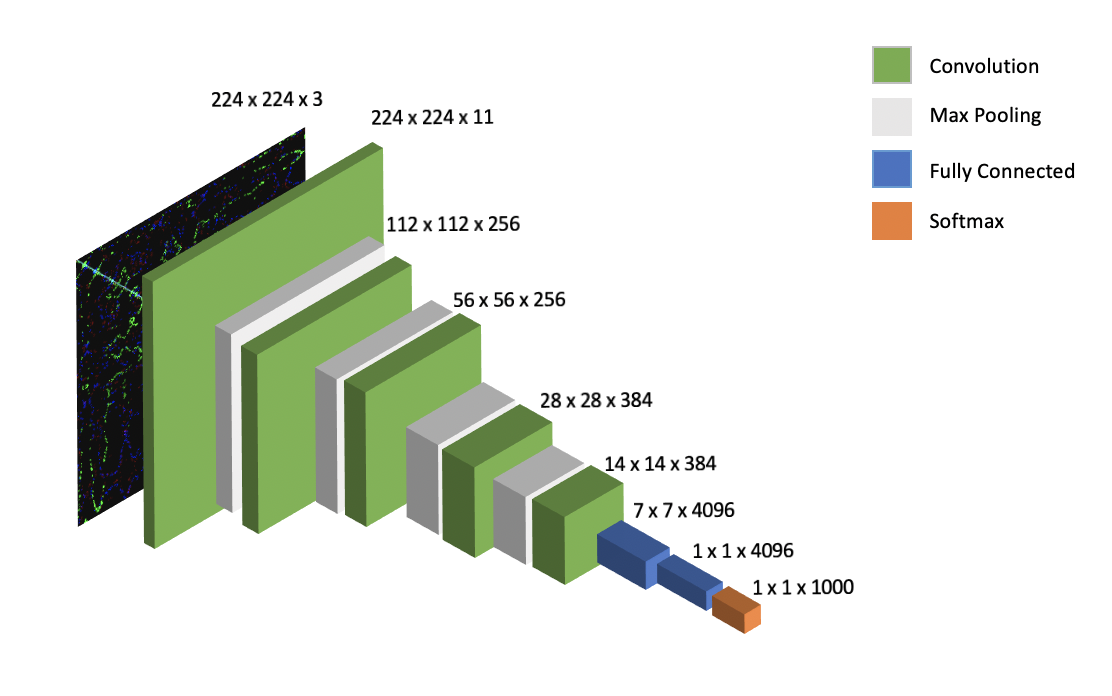
\includegraphics[scale=.7]{../media/2d_cnn.png}
   \end{center}
   \caption{CNN architecture for classifying images generated through MTF.}
   \label{fig:mtf_cnn_model}
\end{figure}

% [add results]


\chapter{Main Results}
\label{chap:results}

\section{Black-Box Model}
Our black-box model is constructed of three different architectures: 1 LSTM and 2 CNN’s that are all concatenated at their respective dense layer (Figure \ref{fig:multimodal_overview}). The three features we use are the amplitude/phase of each level of decomposition for HV. We chose three because we wanted to increase the dimensionality of our data in the event that one had more descriptive features than the others. 

Additionally, we tested our model using three levels of decomposition using the property VV as well as a combination of both VV and HV. We found no change in accuracy, therefore to limit the number of models we used, we only utilized the HV property.


\begin{figure}[h!]
   \begin{center}
      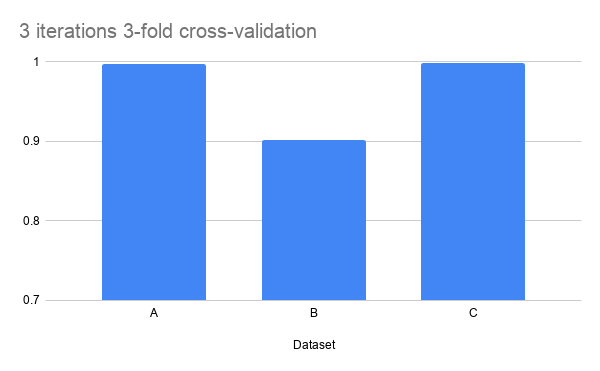
\includegraphics[scale=0.6]{../media/results.png}
   \end{center}
   \caption{Results}
   \label{fig:final_results}
\end{figure}


To test our model, we split our data into training and test sets by randomly selecting 70\% of our data as our training set and leaving the other 30\% to be our test set. We then performed three-fold cross-validation and took the average of our results as the outcome.



\section{Dataset C}

Given that this dataset is ten times larger than our other two datasets, we wanted to try different training and test splits, going as low as 8\% for training data and using the remaining 92\% as test data. We ran the same number of cross-validations as our previous tests and found minimal difference in performance.


% [add table for results]

\section{ MTF }
 
In order to generate images using MTF, we have to select three properties, and we chose P\textsubscript{1} as the radial value of HV's amplitude value, P\textsubscript{2} as the radial value of VV's amplitude value, and P\textsubscript{3} as the absolute squared distance between every P\textsubscript{1} and P\textsubscript{2}. 

We then split those images using a randomized 70/30 split where 70\% of the data is our training set, and the other 30\% is our test set. We were able to achieve 60\% accuracy across all three of our datasets and show the features amongst the classes behave differently, as can be seen in Figure \ref{fig:whitebox_images}.

\begin{figure}[h!]
   \begin{center}
      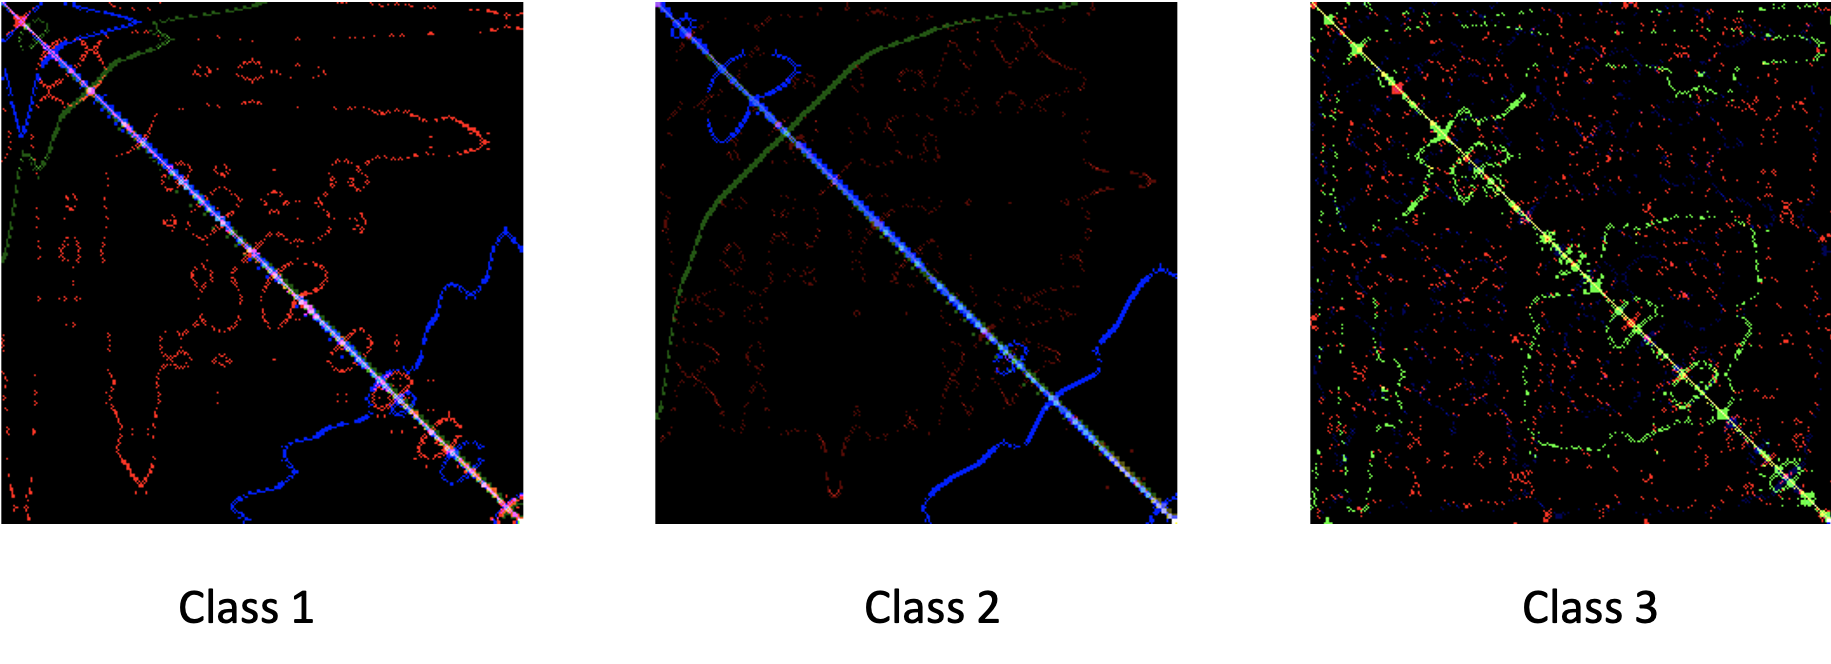
\includegraphics[scale=0.5]{../media/whitebox_images.png}
   \end{center}
   \caption{Examples of images generated through MTF.}
   \label{fig:whitebox_images}
\end{figure}


\chapter{Conclusion}
\label{chap:conclusion}
Throughout this thesis, we have stressed the importance of a hybrid machine learning algorithm as well as provided a framework that can successfully classify and visualize different classes when applied to time-series data. 

We proposed an extension to existing work described in \cite{wang_encoding_nodate} to help users visualize their data while performing classification  with 60\% accuracy on that dataset and model. We also created a robust black-box model consisting of two different deep learning architectures that consistently provided competitive accuracy.

In the future, we would like to explore other methods for our white-box model that would act as an alternative to Markov Transition Fields in hopes that it produces higher accuracy than our current model. Additionally, we would like to extensively test our model on different time-series datasets outside of radio signal datasets.

\begin{appendices}
   \chapter{MTF Code}
      \section{Main File}
         \lstinputlisting[language=Python,  basicstyle=\small, columns=fullflexible ]{../code/mtf/main.py}
      \section{Calculating MTF}
         \lstinputlisting[language=Python,  basicstyle=\small, columns=fullflexible]{../code/mtf/complex_signal.py}
      \section{Helper functions}
         \lstinputlisting[language=Python,  basicstyle=\small, columns=fullflexible]{../code/mtf/util.py}
   \chapter{Hybrid Model Code}
      \section{Main File}
         \lstinputlisting[language=Python,  basicstyle=\small, columns=fullflexible]{../code/hybrid_model/main.py}
      \section{White-Box Model}
         \lstinputlisting[language=Python,  basicstyle=\small, columns=fullflexible]{../code/hybrid_model/white_box.py}
      \section{Black-Box Model}
         \lstinputlisting[language=Python,  basicstyle=\small, columns=fullflexible]{../code/hybrid_model/black_box.py}





\end{appendices}


\bibliography{../references/main}
\bibliographystyle{plain} 

\end{document}
